% !TeX program = lualatex
\documentclass[
	english,
	sections numbered,
	xcolor=dvipsnames,
	aspectratio=169,
]{beamer}

\usepackage{babel}
\usepackage[babel]{microtype}
\usepackage[babel]{csquotes}
\usepackage[american]{isodate}

\usepackage[T1]{fontenc}
\usepackage{FiraMono}

\usetheme[progressbar=frametitle]{metropolis}

%%% GRAPHICS %%%
\usepackage{graphicx}
\usepackage{pgfplots}
\usepackage{tikz}

%%% MATH & SCIENCE %%%
\usepackage{amsmath}
\usepackage{amssymb}
\usepackage{amsfonts}
\usepackage{amsthm}
\usepackage{siunitx}
\usepackage{bm}
\usepackage{dsfont}
\usepackage{mathtools}

%%% FLOATS %%%
\usepackage{booktabs}
\usepackage{tabularx}

%\usepackage{biblatex}
%\bibliography{literature.bib}

\usepackage{appendixnumberbeamer}

% DESIGN COLORS
\definecolor{accent}{HTML}{7EBDC2} % accent color
\definecolor{bgcolor}{HTML}{FCFCFF} % background color
\definecolor{bgcolorAlt}{HTML}{ECF1FC} % alternative background color
\definecolor{fgcolor}{HTML}{222244} % foreground/text color

%
\setbeamercolor{normal text}{%
	fg=fgcolor,
	bg=bgcolor,
}
\setbeamercolor{alerted text}{%
	fg=accent,
}
\setbeamercolor{palette primary}{%
	use=normal text,
	fg=normal text.fg,
	bg=bgcolorAlt,%normal text.bg
}

\setbeamercolor{block title}{
	bg=bgcolorAlt,
}
\setbeamercolor{block body}{
	bg=bgcolorAlt,
}
\setbeamercolor{block title alerted}{%
	use={palette primary, alerted text},
	fg=palette primary.bg,
	bg=alerted text.fg
}
\setbeamercolor{block title example}{%
	use={block title, alerted text},
	bg=block title.bg,
	fg=alerted text.fg
}
%

% PLOT COLORS
%% Paul Tol High Contrast
\definecolor{plot0}{HTML}{004488}
\definecolor{plot1}{HTML}{DDAA33}
\definecolor{plot2}{HTML}{BB5566}
\definecolor{plot3}{HTML}{000000}
\definecolor{plot4}{HTML}{AAAAAA}

%% Paul Tol Vibrant
%\definecolor{plot0}{HTML}{EE7733}
%\definecolor{plot1}{HTML}{0077BB}
%\definecolor{plot2}{HTML}{33BBEE}
%\definecolor{plot3}{HTML}{EE3377}
%\definecolor{plot4}{HTML}{CC3311}
%\definecolor{plot5}{HTML}{009988}
%\definecolor{plot6}{HTML}{BBBBBB}
\setbeamerfont{block body reference}{size=\scriptsize}
\setbeamerfont{block title reference}{size=\scriptsize}

\setbeamerfont{description item}{series=\mdseries}
\setbeamerfont{alerted text}{series=\bfseries\boldmath}

\setbeamerfont{bibliography item}{size=\small}
\setbeamerfont{bibliography entry author}{shape=\upshape,series=\mdseries,size=\small}
\setbeamerfont{bibliography entry title}{shape=\itshape,series=\mdseries,size=\small}
\setbeamerfont{bibliography entry journal}{shape=\upshape,series=\mdseries,size=\small}
\setbeamerfont{bibliography entry location}{shape=\upshape,series=\mdseries,size=\small}
\setbeamerfont{bibliography entry note}{shape=\upshape,series=\mdseries,size=\small}


\setbeamertemplate{title page}{
\begin{minipage}[b][\textheight]{\textwidth}
	\ifx\inserttitlegraphic\@empty\else\usebeamertemplate*{title graphic}\fi
	\vfill%
	\ifx\inserttitle\@empty\else\usebeamertemplate*{title}\fi
	\ifx\insertsubtitle\@empty\else\usebeamertemplate*{subtitle}\fi
	\usebeamertemplate*{title separator}

	\ifx\beamer@shortauthor\@empty\else\usebeamertemplate*{author}\fi
	\ifx\insertdate\@empty\else\usebeamertemplate*{date}\fi
	\ifx\insertinstitute\@empty\else\usebeamertemplate*{institute}\fi
	\vfil
	\vspace*{1mm}
\end{minipage}
}
\newcommand*{\seprule}{{\par\color{bgcolorAlt!90!fgcolor}\hrulefill\par\vspace*{1ex plus 0pt minus .5ex}}}
% Mathematical Writing
\DeclarePairedDelimiter{\abs}{\vert}{\vert}
\DeclarePairedDelimiter{\norm}{\Vert}{\Vert}
\DeclarePairedDelimiter{\ceil}{\lceil}{\rceil}
\DeclarePairedDelimiter{\floor}{\lfloor}{\rfloor}

\newcommand*{\inv}[1]{\ensuremath{#1^{-1}}}
\newcommand*{\positive}[1]{\ensuremath{\left[#1\right]^{+}}}

\newcommand*{\diff}{\ensuremath{\mathrm{d}}}
\newcommand*{\imag}{\ensuremath{\mathrm{j}}}
\newcommand*{\e}{\ensuremath{\mathrm{e}}}

\DeclareMathOperator*{\argmax}{arg\,max}
\DeclareMathOperator*{\argmin}{arg\,min}

%% change these to \mathbb, if you do not want to use the dsfont package
\newcommand*{\reals}{\ensuremath{\mathds{R}}} 
\newcommand*{\complexes}{\ensuremath{\mathds{C}}}
\newcommand*{\naturals}{\ensuremath{\mathds{N}}}
%%

\newcommand*{\expect}[2][]{\ensuremath{\mathbb{E}_{#1}\left[#2\right]}}

\newcommand*{\unif}{\ensuremath{\mathcal{U}}}
\newcommand*{\normaldist}{\ensuremath{\mathcal{N}}}


% THEOREMS
\theoremstyle{plain}% default
\newtheorem{thm}{Theorem}%[section]
\newtheorem{lem}{Lemma}
\newtheorem{prop}{Proposition}
\newtheorem{cor}{Corollary}

\pgfplotsset{compat=newest}

\pgfplotsset{legend style={fill=bgcolor,draw=fgcolor}}

\pgfplotscreateplotcyclelist{lineplot cycle}{ %
	{plot0, mark=*, thick, mark options=solid},
	{plot1, mark=triangle*, thick, mark options=solid},
	{plot2, mark=square*, thick, mark options=solid},
	{plot3, mark=diamond*, thick, mark options=solid},
	{plot4, mark=pentagon*, thick, mark options=solid},
}

\pgfplotsset{%
	betterplot/.style={
		width=.93\linewidth,
		height=.5\textheight,
		xlabel near ticks,
		ylabel near ticks,
		cycle list name=lineplot cycle,
		mark options=solid,
		xmajorgrids=true,
		xminorgrids=true,
		ymajorgrids=true,
%		major grid style={dotted},
		grid style={line width=.1pt, draw=gray!20},
		major grid style={line width=.25pt,draw=gray!30},
		legend cell align=left,
		legend style = {
			/tikz/every even column/.append style={column sep=0.33cm}
		},
	},
}
% Workshop-specific helpers (kept separate from the template's setup-*.tex files)
\usetikzlibrary{arrows.meta,positioning,calc}

% Audience-engagement block. Every engagement frame uses this macro, which also
% lets the build check (see WORKSHOP_GUIDE.md) verify the "one per five slides" rule.
%   #1: type of interaction (Poll, Vote, Predict, Discuss, Pair, ...)
%   #2: the prompt shown to the audience
\newcommand{\audience}[2]{%
	\begin{alertblock}{Audience \textbar{} #1}#2\end{alertblock}%
}

% Maths shorthands used throughout
\newcommand*{\Sn}{S}                         % prefix sums
\newcommand*{\indic}[1]{\ensuremath{\mathds{1}\!\left[#1\right]}}
\newcommand*{\cost}{\ensuremath{w}}
\newcommand*{\Bell}{\ensuremath{\mathcal{T}}} % Bellman operator
\DeclareMathOperator{\gc}{gc}                  % grandchildren
\DeclareMathOperator{\ch}{ch}                  % children
\newcommand*{\supnorm}[1]{\ensuremath{\left\lVert #1\right\rVert_\infty}}

% Styles for state-space drawings
\tikzset{
	st/.style={circle,draw=fgcolor,fill=bgcolorAlt,inner sep=0pt,minimum size=4mm,font=\tiny},
	e/.style={-{Stealth[length=1.5mm]},draw=fgcolor!45},
	hl/.style={-{Stealth[length=1.8mm]},draw=accent,line width=1.4pt},
}



\title{Beyond Dynamic Programming}
\subtitle{State spaces, speed-ups, and Bellman's equations}
\author{Your Name}
\institute[]{Your Affiliation}
\date{Workshop}

% The template ships a placeholder logo; enable once you have a real one:
%\titlegraphic{
\includegraphics[height=.17\textheight]{logo.png}}


\begin{document}
\maketitle

\begin{frame}{Outline}
	\setbeamertemplate{section in toc}[sections numbered]
	\tableofcontents[hideallsubsections]
\end{frame}

\section{Dynamic Programming from First Principles}

\begin{frame}{Calibration}
	\audience[Show of hands]{%
		\begin{enumerate}
			\item Have you implemented the convex hull trick or a Li Chao tree?
			\item Can you state the Bellman optimality equation from memory?
			\item Is Dijkstra's algorithm a dynamic program?
		\end{enumerate}
	}
\end{frame}

\begin{frame}{A motivating problem: minimum edit script}
	Given two versions of a file as token sequences $x \in \Sigma^m$ and $y \in \Sigma^n$,
	find a cheapest sequence of edits that turns $x$ into $y$.

	\begin{itemize}
		\item \textbf{delete} a token of $x$ \hfill cost $1$
		\item \textbf{insert} a token of $y$ \hfill cost $1$
		\item \textbf{substitute} a token \hfill cost $1$ (cost $0$ if the tokens already agree)
	\end{itemize}

	\seprule

	Goal: the minimum total cost $\mathrm{ED}(x,y)$, and an optimal script.
\end{frame}

\begin{frame}{State spaces}
	\begin{block}{Definition}
		A \alert{state space} is a weighted digraph $G=(V,E,\cost)$ with source $s$ and target $t$ such that
		solutions correspond to $s\to t$ paths and the objective is the sum of edge weights.
	\end{block}

	\begin{itemize}
		\item A state $v$ summarises a \emph{partial solution}.
		\item \alert{Sufficiency (Markov property):} the feasible completions of $v$, and
		their costs, depend only on $v$, not on the path that reached it.
	\end{itemize}
\end{frame}

\begin{frame}{The edit-distance state space}
	State $(i,j)$: ``$x_{1..i}$ has been transformed into $y_{1..j}$''.
	Source $(0,0)$, target $(m,n)$.
	\[
		\begin{array}{lll}
			(i-1,j)\to(i,j) & \text{delete } x_i & \cost=1\\
			(i,j-1)\to(i,j) & \text{insert } y_j & \cost=1\\
			(i-1,j-1)\to(i,j) & \text{match / substitute} & \cost=\indic{x_i\neq y_j}
		\end{array}
	\]
\end{frame}

\begin{frame}{The state space is a DAG}
	\begin{columns}[T,onlytextwidth]
		\column{0.58\textwidth}
		\centering
		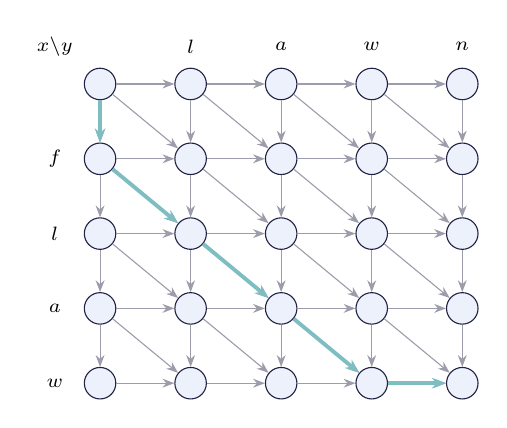
\begin{tikzpicture}[x=1.15cm,y=0.95cm]
			\foreach \i in {0,...,4}{\foreach \j in {0,...,4}{
				\node[st] (n-\i-\j) at (\j,-\i) {};
			}}
			\foreach \i in {1,...,4}{\foreach \j in {0,...,4}{
				\pgfmathtruncatemacro{\ip}{\i-1}
				\draw[e] (n-\ip-\j) -- (n-\i-\j);
			}}
			\foreach \i in {0,...,4}{\foreach \j in {1,...,4}{
				\pgfmathtruncatemacro{\jp}{\j-1}
				\draw[e] (n-\i-\jp) -- (n-\i-\j);
			}}
			\foreach \i in {1,...,4}{\foreach \j in {1,...,4}{
				\pgfmathtruncatemacro{\ip}{\i-1}
				\pgfmathtruncatemacro{\jp}{\j-1}
				\draw[e] (n-\ip-\jp) -- (n-\i-\j);
			}}
			\draw[hl] (n-0-0) -- (n-1-0);
			\draw[hl] (n-1-0) -- (n-2-1);
			\draw[hl] (n-2-1) -- (n-3-2);
			\draw[hl] (n-3-2) -- (n-4-3);
			\draw[hl] (n-4-3) -- (n-4-4);
			\foreach \j/\c in {1/l,2/a,3/w,4/n}{\node[font=\scriptsize] at (\j,0.5) {$\c$};}
			\foreach \i/\c in {1/f,2/l,3/a,4/w}{\node[font=\scriptsize] at (-0.5,-\i) {$\c$};}
			\node[font=\scriptsize] at (-0.5,0.5) {$x\backslash y$};
		\end{tikzpicture}

		\column{0.4\textwidth}
		\begin{itemize}
			\item Every edge increases $i+j$: \alert{acyclic}.
			\item Highlighted: \texttt{flaw} $\to$ \texttt{lawn}, cost $2$.
			\item $(m+1)(n+1)$ states, $\le 3$ in-edges each.
		\end{itemize}
	\end{columns}
\end{frame}

\begin{frame}{Paths versus states}
	\audience[How many edit scripts?]{%
		For $m=n=20$, roughly how many $s\to t$ paths are there?\\[0.5em]
		(a)~$10^{6}$ \quad (b)~$10^{9}$ \quad (c)~$10^{12}$ \quad (d)~$>10^{14}$
	}
\end{frame}

\begin{frame}{Paths versus states: answer}
	The number of paths is the central Delannoy number $D(n,n)\sim c\,(3+2\sqrt2)^n$.
	\begin{center}
		$D(20,20) = 260{,}543{,}813{,}797{,}441 \approx 2.6\cdot 10^{14}$ paths
		\quad versus \quad $(20+1)^2=441$ states.
	\end{center}
	The state graph is a \alert{compressed representation} of the solution space.
\end{frame}

\begin{frame}{Dynamic programming on a DAG}
	\begin{theorem}
		Let $G=(V,E,\cost)$ be a DAG with source $s$, and $d(v)$ the minimum weight of an
		$s\to v$ path ($\infty$ if none). Then
		\[
			d(s)=0, \qquad d(v)=\min_{(u,v)\in E}\bigl\{\,d(u)+\cost(u,v)\,\bigr\}\quad (v\neq s).
		\]
	\end{theorem}
\end{frame}

\begin{frame}{Why it works}
	An $s\to v$ path is an $s\to u$ path followed by an edge $(u,v)$.
	\begin{itemize}
		\item \alert{Optimal substructure.} The choice of prefix does not constrain the last edge,
		so minimising each prefix loses nothing.
		\item \alert{Well-foundedness.} Acyclicity lets us induct along a topological order.
	\end{itemize}
\end{frame}

\begin{frame}{A strategy for dynamic programming problems}
	\begin{enumerate}
		\item \textbf{Decompose.} Choose a state space: what must be remembered about a
		partial solution so that the future is independent of the past?
		\item \textbf{Recurrence.} State the \alert{base case} and the \alert{inductive step}.
		\item \textbf{Evaluate bottom-up} in a topological order of the state DAG.
		\item \textbf{Reconstruct} the solution, if needed, from the minimising predecessor of each state.
	\end{enumerate}
\end{frame}

\begin{frame}{Complexity is read off the DAG}
	\[
		T \;=\; \sum_{v\in V} \bigl(\text{work to evaluate state } v\bigr) \;=\; |V|\times(\text{cost per state}) \;\approx\; |E|.
	\]
\end{frame}

\begin{frame}{Steps 1--2: the recurrence for edit distance}
	Let $f(i,j)$ be the minimum cost of transforming $x_{1..i}$ into $y_{1..j}$.

	\begin{align*}
		\text{base:}\quad & f(i,0)=i, \qquad f(0,j)=j\\[0.3em]
		\text{step:}\quad & f(i,j)=\min\begin{cases}
			f(i-1,j)+1 & \text{delete } x_i\\
			f(i,j-1)+1 & \text{insert } y_j\\
			f(i-1,j-1)+\indic{x_i\neq y_j} & \text{match / substitute}
		\end{cases}
	\end{align*}
	Answer: $\mathrm{ED}(x,y)=f(m,n)$.
\end{frame}

\begin{frame}{Step 3: bottom-up evaluation}
	\audience[Fill in the last two rows]{%
		\centering
		\renewcommand{\arraystretch}{1.15}
		\begin{tabular}{@{}c|ccccc@{}}
			& $\varepsilon$ & \texttt{l} & \texttt{a} & \texttt{w} & \texttt{n}\\
			\midrule
			$\varepsilon$ & 0 & 1 & 2 & 3 & 4\\
			\texttt{f} & 1 & 1 & 2 & 3 & 4\\
			\texttt{l} & 2 & 1 & 2 & 3 & 4\\
			\texttt{a} & ? & ? & ? & ? & ?\\
			\texttt{w} & ? & ? & ? & ? & ?\\
		\end{tabular}
	}
\end{frame}

\begin{frame}{Step 3: bottom-up evaluation, filled in}
	\centering
	\renewcommand{\arraystretch}{1.15}
	\begin{tabular}{@{}c|ccccc@{}}
		& $\varepsilon$ & \texttt{l} & \texttt{a} & \texttt{w} & \texttt{n}\\
		\midrule
		$\varepsilon$ & 0 & 1 & 2 & 3 & 4\\
		\texttt{f} & 1 & 1 & 2 & 3 & 4\\
		\texttt{l} & 2 & 1 & 2 & 3 & 4\\
		\texttt{a} & 3 & 2 & \alert{1} & 2 & 3\\
		\texttt{w} & 4 & 3 & 2 & \alert{1} & \alert{2}\\
	\end{tabular}

	\vspace{1em}
	$\mathrm{ED}(\texttt{flaw},\texttt{lawn})=f(4,4)=2$.
\end{frame}

\begin{frame}{Step 4: reconstruction}
	Walk back from $(m,n)$ along minimising predecessors:
	\[
		(4,4)\xleftarrow{\text{insert n}}(4,3)\xleftarrow{\text{match w}}(3,2)\xleftarrow{\text{match a}}(2,1)\xleftarrow{\text{match l}}(1,0)\xleftarrow{\text{delete f}}(0,0).
	\]
	\begin{center}
		\ttfamily
		\begin{tabular}{@{}cccccc@{}}
			f & l & a & w & - \\
			- & l & a & w & n \\
			\textrm{del} & = & = & = & \textrm{ins}
		\end{tabular}
	\end{center}
\end{frame}

\begin{frame}{Memory}
	\begin{itemize}
		\item The value table costs $\Theta(mn)$ memory; the argmin can be recomputed from it.
		\item Rolling two rows: $\Theta(\min(m,n))$ memory, but no reconstruction.
		\item \alert{Hirschberg's divide-and-conquer}: reconstruction in linear space at twice the time.
	\end{itemize}
\end{frame}

\begin{frame}{Complexity and its limits}
	$|V|=(m+1)(n+1)$, at most $3$ predecessors each: $\Theta(mn)$ time.

	\begin{itemize}
		\item \textbf{Output-sensitive.} If $\mathrm{ED}\le d$, only the band $|i-j|\le d$ matters:
		$O(d\cdot\min(m,n))$ (Ukkonen); Myers' $O(nd)$ diff is the engine behind \texttt{git diff}.
		\item \textbf{Lower bound.} No $O(n^{2-\varepsilon})$ algorithm exists unless SETH
		fails (Backurs--Indyk, STOC 2015).
	\end{itemize}
\end{frame}

\begin{frame}{Is the state space really sufficient?}
	\audience[Adding transpositions]{%
		Allow \textbf{transpositions} of adjacent tokens ($ab\to ba$) at cost $1$.
		\begin{enumerate}
			\item Which edge do you add to the DAG, and when?
			\item Does the complexity change?
			\item Is the result exactly the Damerau--Levenshtein distance?
		\end{enumerate}
	}
\end{frame}

\begin{frame}{Transpositions: the edge}
	\begin{enumerate}
		\item Add $(i-2,j-2)\to(i,j)$ with cost $1$ when $x_i=y_{j-1}$ and $x_{i-1}=y_j$.
		\item Still $\Theta(mn)$: one more $O(1)$ in-edge per state.
	\end{enumerate}
\end{frame}

\begin{frame}{Transpositions: not Damerau--Levenshtein}
	\begin{enumerate}
		\setcounter{enumi}{2}
		\item \alert{No.} This computes the \emph{optimal string alignment} distance, in which no substring is edited twice.
	\end{enumerate}

	\vspace{0.5em}
	For $x=\texttt{CA}$, $y=\texttt{ABC}$ it gives $3$.
	The true distance is $2$: \texttt{CA}$\to$\texttt{AC}$\to$\texttt{ABC}.

	\seprule

	The state space is \alert{not sufficient}. The exact algorithm needs edges reaching back to the
	last occurrence of a symbol (see backup).
\end{frame}

\begin{frame}{Part 1 in one slide}
	What made this a dynamic program?
	\begin{enumerate}
		\item \textbf{A sufficient state}, giving a graph that compresses exponentially many solutions.
		\item \textbf{Acyclicity}, giving a well-founded order of evaluation.
		\item \textbf{Additive (or otherwise decomposable) objective}, giving optimal substructure.
	\end{enumerate}

	\seprule

	\textbf{Design is in step 1.} Steps 2--4 and the complexity follow mechanically.
\end{frame}

\section{Is It Dynamic Programming? Case Studies}

\begin{frame}{How this part works}
	For each problem you will see \alert{candidate solutions}. Your job is to decide:
	\begin{enumerate}
		\item Is it \textbf{correct}?
		\item Is it \textbf{the right tool}?
	\end{enumerate}

	\seprule

	\textbf{Triage test for dynamic programming}
	\begin{enumerate}
		\item Is there a \emph{sufficient} state of polynomial size? (Markov property)
		\item Does the objective decompose over it? (optimal substructure)
		\item Is there no cheaper algorithm that exploits more structure?
	\end{enumerate}
	A positive answer to (1) and (2) makes DP \emph{correct}; (3) decides whether it is \emph{good}.
\end{frame}

\begin{frame}{Case 1: Split Array Largest Sum (LeetCode 410)}
	Given $a_1,\dots,a_n\ge 0$ and $k\le n$, split the array into $k$ non-empty
	contiguous parts so as to \alert{minimise the largest part sum}. Let $S_i=\sum_{l\le i}a_l$.

	\seprule

	\textbf{Example.} $a=(7,2,5,10,8)$, $k=2$: the parts $(7,2,5)\,|\,(10,8)$ give $\max\{14,18\}=18$, which is optimal.

	\vspace{1em}
	We will look at two proposals.
\end{frame}

\begin{frame}{Case 1: candidate solutions}
	\begin{columns}[T,onlytextwidth]
		\column{0.52\textwidth}
		\begin{block}{Proposal A (recurrence)}
			\small
			Let $f(i,j)$ be the best value for the first $i$ elements in $j$ parts.
			\begin{align*}
				f(0,0)&=0, \quad f(i,0)=f(0,j)=\infty\\
				f(i,j)&=\min_{j-1\le p<i}\max\bigl\{f(p,j-1),\;S_i-S_p\bigr\}
			\end{align*}
			Answer $f(n,k)$.
		\end{block}

		\column{0.44\textwidth}
		\begin{block}{Proposal B (greedy)}
			\small
			Let $\bar S=\lceil S_n/k\rceil$. Sweep left to right and close the current part
			as soon as adding the next element would exceed $\bar S$ (until $k-1$ parts are closed).
		\end{block}
	\end{columns}

	\audience{Vote}{%
		For each proposal: \textbf{correct} or \textbf{incorrect}? And if correct, is it \textbf{efficient}?
	}
\end{frame}

\begin{frame}{Case 1: verdict}
	\begin{columns}[T,onlytextwidth]
		\column{0.5\textwidth}
		\textbf{A is correct.} The state $(i,j)$ is sufficient (only the prefix length and number of parts matter),
		and $(\max,\min)$ composes. But the cost:
		\[
			\underbrace{nk}_{\text{states}}\times\underbrace{O(n)}_{\text{per state}}=\Theta(kn^2).
		\]

		\column{0.46\textwidth}
		\textbf{B is wrong.} Take $a=(1,3,2)$, $k=2$: $\bar S=3$, so B closes $(1)$ and returns $(1)\,|\,(3,2)$ with
		value $5$, while $(1,3)\,|\,(2)$ achieves $4$.
	\end{columns}

	\seprule

	Greedy heuristics that ``balance'' parts fail because the objective is the \emph{maximum}, not a
	deviation from the mean. Is there a correct greedy at all?
\end{frame}

\begin{frame}{Case 1: a better algorithm, and why DP is wasteful}
	\small
	\textbf{Decide, then optimise.} For a cap $L$ let $c(L)$ be the minimum number of parts
	with every sum $\le L$. The greedy ``extend each part as far as possible'' computes $c(L)$ in $O(n)$
	(it stays ahead of any other partition).

	\begin{itemize}
		\item $c$ is non-increasing in $L$; since $k\le n$, a partition into fewer parts can always be refined.
		\item The answer is $\min\{L\in[\max_i a_i,\,S_n]\;:\;c(L)\le k\}$, found by binary search.
	\end{itemize}
	\vspace{0.3em}
	\begin{center}
		\begin{tabular}{@{}lc@{}}
			\toprule
			Method & Time\\
			\midrule
			Proposal A & $\Theta(kn^2)$\\
			A with monotone optimum (binary search over $p$) & $O(kn\log n)$\\
			Binary search on the answer + greedy & $O(n\log S_n)$\\
			\bottomrule
		\end{tabular}
	\end{center}
	DP computes $f(i,j)$ for \emph{every} prefix and part count, but we need one number.
\end{frame}

\begin{frame}{Case 1: discussion}
	\audience{Discuss}{%
		\begin{enumerate}
			\item Which property of ``minimise the \emph{maximum}'' made the decision version
			greedy-checkable and monotone in $L$?
			\item Suppose we instead minimise the \textbf{sum of squares} of part sums. Does binary search
			on the answer still work? What would you use?
		\end{enumerate}
	}

	\uncover<2->{%
		\small
		\begin{enumerate}
			\item The max commutes with refinement: splitting a part never increases the objective,
			and feasibility under a cap is local.
			\item No: there is no threshold structure. This is a genuine DP,
			$f(i,j)=\min_p f(p,j-1)+(S_i-S_p)^2$, and its transition has the form that the
			\alert{convex hull trick} exploits in Part~3.
		\end{enumerate}
	}
\end{frame}

\begin{frame}{Case 2: Maximum weight independent set on a tree}
	LeetCode 337 (\emph{House Robber III}); the path case is LeetCode 198.

	Tree $T=(V,E)$ rooted at $r$, weights $w_v\ge0$. Choose an independent set $I$ maximising $\sum_{v\in I}w_v$.
	Write $\ch(v)$ for the children and $\gc(v)$ for the grandchildren of $v$.

	\seprule

	\begin{itemize}
		\item For general graphs the problem is NP-hard.
		\item On a tree, the subtree of $v$ is separated from the rest of the tree by the single vertex $v$.
	\end{itemize}

	\begin{center}
		Where would you put the state?
	\end{center}
\end{frame}

\begin{frame}{Case 2: candidate solutions}
	\small
	\begin{description}
		\item[\alert{Proposal A}] Greedy: repeatedly take the heaviest remaining vertex and delete its neighbours.
		\item[\alert{Proposal B}] $f(v)=\max\bigl\{\,w_v+\sum_{c\in\ch(v)}f(c),\;\sum_{c\in\ch(v)}f(c)\bigr\}$
		\item[\alert{Proposal C}] $f(v)=\max\bigl\{\,w_v+\sum_{g\in\gc(v)}f(g),\;\sum_{c\in\ch(v)}f(c)\bigr\}$
		\item[\alert{Proposal D}] $f(v,1)=w_v+\sum_{c}f(c,0)$ and $f(v,0)=\sum_c\max\{f(c,0),f(c,1)\}$; answer $\max_b f(r,b)$.
	\end{description}

	\audience{Vote}{%
		Which proposals are \textbf{correct}? Look for a counterexample for those you reject.
	}
\end{frame}

\begin{frame}{Case 2: verdict}
	\small
	\begin{columns}[T,onlytextwidth]
		\column{0.5\textwidth}
		\textbf{A and B are wrong.} Path $2-3-2$:
		\begin{itemize}
			\item A takes the centre: value $3$; optimum $4$ (both ends).
			\item B, rooted at the centre: $f(\text{leaf})=2$, so $f(\text{root})=\max\{3+4,4\}=7$.
			The term $w_v+\sum_c f(c)$ forgets that $f(c)$ may itself use $c$.
		\end{itemize}

		\column{0.46\textwidth}
		\textbf{C and D are correct.} In D the state records whether $v$ is chosen:
		\begin{align*}
			f(v,1)&=w_v+\sum_{c}f(c,0)\\
			f(v,0)&=\sum_{c}\max_b f(c,b)
		\end{align*}
		C is D with the state projected out: $f(v)=\max_b f(v,b)$.
	\end{columns}

	\seprule

	Time $\Theta(\sum_v\deg v)=\Theta(n)$. Both formulations have the same state DAG (the rooted tree), but
	D carries $2n$ states and has \emph{local} transitions. Enlarging the state to make the transition local is a standard trick.
\end{frame}

\begin{frame}{Case 2: why trees, and what generalises}
	The tree makes $v$ a \alert{separator}: the two sides interact only through $v$'s status.

	\begin{theorem}[folklore]
		Given a tree decomposition of width $\omega$ of an $n$-vertex graph, a maximum weight independent
		set can be computed in $O(2^{\omega}\,\omega\, n)$ time.
	\end{theorem}
	The state of a bag is the independent subset chosen inside it ($\le 2^{\omega+1}$ states);
	the structure of the graph \emph{is} the shape of the state DAG.

	\seprule

	\textbf{Same recipe, different shape.}
	Trees ($\omega=1$), cycles ($\omega=2$), series-parallel graphs ($\omega\le2$), grids $k\times n$ ($\omega=k$).
\end{frame}

\begin{frame}{Case 2: discussion}
	\audience{Discuss}{%
		Now let the graph be a \textbf{cycle} $C_n$ with weights $w_1,\dots,w_n$.
		The tree recurrence is no longer valid. Fix it, and give the complexity.
	}

	\uncover<2->{%
		\small
		Fix the status $b_1$ of vertex $1$ and run the path DP on $1,\dots,n$ with that boundary condition
		(for $b_1=1$ vertex $n$ is forbidden): two path DPs, $\Theta(n)$ in total.
		Equivalently, enlarge the state to $(b_1,b_{\text{current}})$: this is the width-$2$ tree decomposition
		made explicit, with $4$ states per position.
	}
\end{frame}

\begin{frame}{Case 3: Minimum Initial Energy to Finish Tasks (LeetCode 1665)}
	Tasks $i=1,\dots,n$ with $(a_i,m_i)$, $a_i\le m_i$: to \emph{start} task $i$ you need at least $m_i$ energy,
	and finishing it consumes $a_i$. Choose the order $\pi$ and the initial energy $E$ to finish all tasks, minimising $E$.

	\seprule

	For an order $\pi$:
	\[
		E(\pi)=\max_{t}\Bigl(m_{\pi(t)}+\sum_{s<t}a_{\pi(s)}\Bigr),\qquad
		E^\star=\min_{\pi}E(\pi).
	\]
	The order is a free choice. There are $n!$ orders.

	\begin{center}
		It looks like a perfect candidate for DP: a sequence of decisions, additive consumption.
	\end{center}
\end{frame}

\begin{frame}{Case 3: candidate solutions}
	Let $A(S)=\sum_{i\in S}a_i$.
	\small
	\begin{description}
		\item[\alert{Proposal A}] Sort by $m_i$ in \emph{decreasing} order and do tasks in that order.
		\item[\alert{Proposal B}] Sort by $a_i$ in \emph{increasing} order.
		\item[\alert{Proposal C}] $F(\emptyset)=0$, $\;F(S)=\min_{i\in S}\max\bigl\{F(S\setminus\{i\}),\;A(S\setminus\{i\})+m_i\bigr\}$; answer $F([n])$.
	\end{description}

	\audience{Vote}{%
		Correct or incorrect? Is C a ``dynamic programming solution''? Is it a \emph{useful} one?
	}
\end{frame}

\begin{frame}{Case 3: verdict}
	\small
	Tasks written $[a_i,m_i]$.
	\begin{itemize}
		\item \textbf{A is wrong:} $[1,2],[3,3]$. A runs $[3,3]$ first and needs $\max\{3,\,3+2\}=5$;
		running $[1,2]$ first needs $\max\{2,\,1+3\}=4$.
		\item \textbf{B is wrong:} $[1,1],[2,3]$. B needs $\max\{1,1+3\}=4$; the other order needs $\max\{3,2+1\}=3$.
		\item \textbf{C is correct.} The energy left after finishing a set $S$ is $E-A(S)$ \emph{whatever the order}, so
		the set is a sufficient state.
	\end{itemize}

	\seprule

	But the state is the \alert{whole subset}: $2^n$ states, $\Theta(2^nn)$ time. No polynomial-size sufficient state
	is apparent: the future depends on \emph{which} tasks remain, not on a number summarising them.
	This is the sense in which the DP is a false positive: the formulation is valid, but the state does not compress.
\end{frame}

\begin{frame}{Case 3: what actually solves it}
	\small
	\textbf{Key} $\kappa_i=m_i-a_i$. \alert{Claim:} an order sorted by decreasing $\kappa$ is optimal.

	\begin{proof}[Exchange argument]
		Suppose $i$ is run immediately before $j$ with $\kappa_i\ge\kappa_j$ versus the swapped order,
		with identical energy before and after the pair. Then
		\begin{align*}
			E(i,j)&=\max\{a_i+\kappa_i,\;a_i+a_j+\kappa_j\}\\
			&\le a_i+a_j+\kappa_i\le \max\{m_j,\;a_j+m_i\}=E(j,i).
		\end{align*}
		Any order with an adjacent pair violating $\kappa_i\ge\kappa_j$ is therefore no better than
		the order with the pair swapped; repeated swaps sort the sequence (bubble sort) without increasing the requirement.
	\end{proof}

	Time $O(n\log n)$. The structure that makes this problem easy is an \alert{exchange argument}, not a state space.
\end{frame}

\begin{frame}{Rapid fire: DP, or not?}
	\audience{Vote}{%
		For each: \textbf{DP}, \textbf{something better}, or \textbf{no compact DP}?
	}
	\small
	\begin{enumerate}
		\item Minimum number of coins summing to $V$.
		\item Unweighted interval scheduling (maximum number of disjoint intervals).
		\item Longest \emph{simple} path in a general directed graph.
		\item $0/1$ knapsack with $n=40$ items and weights up to $10^{12}$.
		\item Longest increasing subsequence.
		\item Shortest paths in a graph with cycles and non-negative weights.
	\end{enumerate}
\end{frame}

\begin{frame}{Rapid fire: answers}
	\small
	\begin{enumerate}
		\item \textbf{DP.} State $=$ remaining amount.
		\item \textbf{Something better.} Earliest-finish-time greedy ($O(n\log n)$); DP is valid but unnecessary.
		\item \textbf{No compact DP.} NP-hard; subset DP is $\Theta(2^nn)$, the state has to record the visited set.
		\item \textbf{Something better.} $O(nW)$ is hopeless; meet-in-the-middle gives $O(2^{n/2}\,n)$.
		\item \textbf{DP, then better.} $O(n^2)$ DP; changing the state to \emph{(length $\to$ smallest tail)}
		gives $O(n\log n)$ by patience sorting.
		\item \textbf{DP in disguise.} The Bellman equations hold but are cyclic; Dijkstra chooses an
		evaluation order. This is the theme of Part~4.
	\end{enumerate}
\end{frame}

\section{Going Faster}

\begin{frame}{Where does the time go?}
	Time $\approx\sum_v \text{indeg}(v)=|E|$. Two levers, both about the \emph{shape} of the DAG, not its meaning:

	\begin{enumerate}
		\item[\alert{I}] \textbf{Change the recurrence.} Algebra on the transition turns
		``minimum over all predecessors'' into a structured query (a data-structure operation).
		\item[\alert{II}] \textbf{Change the compute order.} Refine the DAG with intermediate states so
		that every state has $O(1)$ in-edges, computing the same values.
	\end{enumerate}

	\seprule

	We illustrate (I) with the \textbf{convex hull trick} and (II) with a \textbf{bitmask profile DP}.
\end{frame}

\begin{frame}{Lever I: a problem with a quadratic transition}
	\textbf{Batched jobs.} Jobs $1,\dots,n$ must be processed in order; job $l$ has size $c_l\ge0$ and $S_i=\sum_{l\le i}c_l$.
	Partition the sequence into consecutive batches. A batch of total size $s$ costs $M+s^2$ (set-up plus a quadratic penalty).

	Let $\mathrm{dp}(i)$ be the optimal cost for the first $i$ jobs:
	\[
		\mathrm{dp}(0)=0,\qquad
		\mathrm{dp}(i)=\min_{0\le j<i}\Bigl\{\,\mathrm{dp}(j)+(S_i-S_j)^2+M\,\Bigr\}.
	\]

	$n$ states, $\Theta(n)$ predecessors each: $\Theta(n^2)$. For $n=10^6$ that is hopeless.

	\audience{Discuss}{%
		Expand the square. \textbf{Which terms couple $i$ and $j$?}
		What does that suggest about the inner minimisation?
	}
\end{frame}

\begin{frame}{Rewriting the recurrence}
	\small
	\[
		\mathrm{dp}(i)=S_i^2+M+\min_{j<i}\Bigl\{\underbrace{(-2S_j)}_{m_j}\cdot S_i+\underbrace{\mathrm{dp}(j)+S_j^2}_{b_j}\Bigr\}.
	\]
	Only the cross term $-2S_iS_j$ couples $i$ and $j$. Everything else is a function of $i$ alone or of $j$ alone.

	\seprule

	Define the line $\ell_j(x)=m_jx+b_j$. Then
	\[
		\boxed{\;\mathrm{dp}(i)=S_i^2+M+\min_{j<i}\ell_j(S_i)\;}
	\]
	The inner term is the \alert{lower envelope} of the lines $\ell_0,\dots,\ell_{i-1}$ evaluated at $S_i$.
	The line $\ell_i$ becomes available only after $\mathrm{dp}(i)$ is known (an \emph{online} insertion).
\end{frame}

\begin{frame}{The lower envelope}
	\centering
	\begin{tikzpicture}
		\begin{axis}[
			betterplot,
			width=0.62\textwidth, height=5.6cm,
			xmin=0,xmax=5,ymin=-3.5,ymax=8,
			xlabel={$x$}, ylabel={$\ell_j(x)$},
			legend pos=south west, legend style={font=\scriptsize},
			cycle list name=lineplot cycle,
			]
			\addplot[domain=0:5,thick,plot0,no marks] {6};
			\addplot[domain=0:5,thick,plot1,no marks,dashed] {7-x};
			\addplot[domain=0:5,thick,plot2,no marks] {6.9-1.5*x};
			\addplot[domain=0:5,thick,plot3,no marks] {12-3*x};
			\addplot[domain=0:0.6,very thick,accent,no marks] {6};
			\addplot[domain=0.6:3.4,very thick,accent,no marks] {6.9-1.5*x};
			\addplot[domain=3.4:5,very thick,accent,no marks] {12-3*x};
			\legend{$\ell_0$,$\ell_1$ (redundant),$\ell_2$,$\ell_3$}
		\end{axis}
	\end{tikzpicture}

	\small Slopes decrease with insertion order ($m_j=-2S_j$, $S_j$ non-decreasing), so each new line
	is the best one for \emph{large} $x$. The dashed line never attains the minimum and may be discarded.
\end{frame}

\begin{frame}{The monotone convex hull trick}
	\small
	Keep the envelope as a deque $Q$ of lines in insertion order; queries $S_i$ are non-decreasing.

	\begin{enumerate}
		\item \textbf{Query.} While $|Q|\ge2$ and $\ell_{Q_2}(S_i)\le\ell_{Q_1}(S_i)$, pop the front.
		Then $\mathrm{dp}(i)=S_i^2+M+\ell_{Q_1}(S_i)$.
		\item \textbf{Insert} $\ell_i$. While $|Q|\ge2$ and the last line $\ell_2$ (predecessor $\ell_1$; slopes $m_1>m_2>m_i$) is redundant, pop the back:
		\[
			\ell_2\text{ redundant}\iff (b_i-b_1)(m_1-m_2)\le(b_2-b_1)(m_1-m_i),
		\]
		i.e.\ $\ell_1,\ell_i$ intersect left of $\ell_1,\ell_2$.
	\end{enumerate}

	\seprule

	Each line is pushed once and popped at most once: \alert{amortised $O(1)$ per state, $\Theta(n)$ in total}.
	The front can be discarded because later queries are larger and later lines have smaller slopes.
\end{frame}

\begin{frame}{Robustness of the trick}
	\small
	\audience{Vote}{%
		The data are \textbf{not monotone}. Choose the data structure.
		(a)~Slopes inserted in decreasing order, \emph{arbitrary} query points.
		(b)~\emph{Arbitrary} slopes (e.g.\ some $c_l<0$), arbitrary queries, online.
	}

	\uncover<2->{%
		\begin{enumerate}
			\item[(a)] Keep the hull as an array and \alert{binary-search} the query: $O(n\log n)$ total.
			\item[(b)] A \alert{Li Chao tree} over the query domain (or a dynamic hull): $O(\log C)$ per insertion and query
			($C$ = size of the query domain; compress coordinates offline if needed).
		\end{enumerate}
		Implementation note: the redundancy test multiplies differences of intercepts and slopes; for $S\sim10^{9}$ the products need $128$-bit arithmetic.
	}
\end{frame}

\begin{frame}{What structure was exploited?}
	\small
	The trick applies whenever the transition separates as
	$\mathrm{dp}(i)=\alpha_i+\min_{j<i}\{\beta_j+\gamma_i\,\delta_j\}$. Other structure in $\mathrm{cost}(j,i)$ gives other accelerations:

	\footnotesize
	\begin{center}
		\renewcommand{\arraystretch}{1.15}
		\begin{tabular}{@{}p{0.31\textwidth}p{0.4\textwidth}p{0.18\textwidth}@{}}
			\toprule
			Structure of $\mathrm{cost}(j,i)$ & Technique & Gain\\
			\midrule
			Separable (inner product) & Convex hull trick / Li Chao tree & $n^2\to n,\;n\log n$\\
			Monge, 1D/1D online & Monotone optimum; SMAWK, LARSCH & $n^2\to n\log n$ or $n$\\
			Monge, $k$ layers & Divide-and-conquer optimisation & $kn^2\to kn\log n$\\
			Convex in number of layers $k$ & Lagrangian relaxation (``Aliens trick'') & removes factor $k$\\
			Interval DP, monotone optimum & Knuth--Yao & $n^3\to n^2$\\
			\bottomrule
		\end{tabular}
	\end{center}
\end{frame}

\begin{frame}{Lever II: tilings and bitmask DP}
	\small
	\textbf{Floorplanning.} Count the tilings of an $n\times m$ board (some cells may be blocked) by $1\times2$ dominoes, with $m$ small ($\le 16$) and $n$ large.

	\textbf{Row-by-row.} Let $G_r(M')$ count partial tilings in which rows $<r$ are fully covered and
	$M'\subseteq\{0,\dots,m-1\}$ are exactly the cells of row $r$ covered by vertical dominoes from row $r-1$.
	\[
		G_0(\emptyset)=1,\qquad
		G_{r+1}(M')=\sum_{M\;\text{compatible with}\;M'}G_r(M),\qquad\text{answer }G_n(\emptyset).
	\]
	$M$ and $M'$ are compatible iff $M\cap M'=\emptyset$ and the cells of the row outside $M\cup M'$ split into
	runs of even length (to be tiled by horizontal dominoes).

	\seprule

	$2^m$ states per row. Compatible pairs: up to $3^m$. Time $\Theta(n\,3^m)$.
\end{frame}

\begin{frame}{The edge count is the bottleneck}
	\audience{Discuss}{%
		There are only $2^m$ states per row, but $3^m$ edges between consecutive rows.
		Can the \textbf{same} counts be computed with fewer edges?
		\emph{Hint:} what if we decide one cell at a time?
	}

	\uncover<2->{%
		\small
		Insert intermediate states between rows: process cells in row-major order and keep, as state, the
		\alert{profile} of the next $m$ cells (already covered or not). Each cell has $O(1)$ choices: skip, place a
		vertical domino, place a horizontal domino. Same sums, regrouped; edges per state drop from $2^m$ to $O(1)$.
	}
\end{frame}

\begin{frame}{Broken profile DP}
	\small
	Number cells $t=rm+c$ in row-major order. Let $F_t(M)$, $M\in\{0,1\}^m$, count partial tilings in which cells $<t$ are
	covered, and bit $k$ of $M$ says whether cell $t+k$ is already covered.
	\[
		F_0(0)=1,\qquad \text{answer }F_{nm}(0).
	\]
	From $F_t(M)$, with cell $t=(r,c)$:
	\begin{align*}
		M_0=1:\;& F_{t+1}\bigl(M\gg1\bigr)\mathrel{+}=F_t(M)\\
		M_0=0:\;& F_{t+1}\bigl((M\gg1)\,|\,2^{m-1}\bigr)\mathrel{+}=F_t(M) && \text{vertical, if } r+1<n\\
		M_0=M_1=0:\;& F_{t+1}\bigl((M\gg1)\,|\,1\bigr)\mathrel{+}=F_t(M) && \text{horizontal, if } c+1<m
	\end{align*}
	Blocked cells: forbid dominoes that would cover them and let a blocked cell pass through unchanged.

	\seprule

	States: $nm\,2^m$. In-edges: $\le 3$. Time $\Theta(nm\,2^m)$ versus $\Theta(n\,3^m)$.
\end{frame}

\begin{frame}{Same values, different DAG}
	\centering
	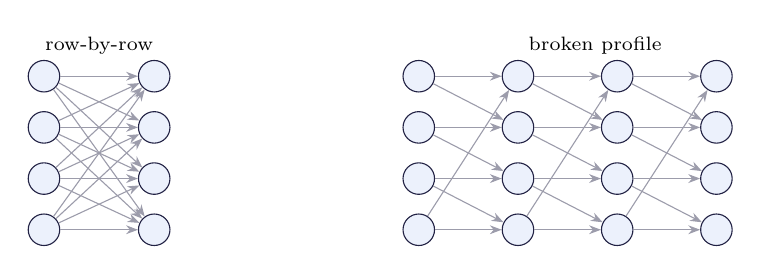
\begin{tikzpicture}[x=1.4cm,y=0.65cm]
		% left: dense layer to layer
		\node[font=\scriptsize] at (0.5,2.1) {row-by-row};
		\foreach \a in {0,1,2,3}{\node[st] (a\a) at (0,-\a+1.5) {};}
		\foreach \b in {0,1,2,3}{\node[st] (b\b) at (1,-\b+1.5) {};}
		\foreach \a in {0,1,2,3}{\foreach \b in {0,1,2,3}{\draw[e] (a\a) -- (b\b);}}
		% right: chain of sparse layers
		\node[font=\scriptsize] at (5,2.1) {broken profile};
		\foreach \k in {0,1,2,3}{
			\foreach \a in {0,1,2,3}{\node[st] (c\k\a) at (3.4+0.9*\k,-\a+1.5) {};}
		}
		\foreach \k/\kk in {0/1,1/2,2/3}{
			\foreach \a/\b in {0/0,0/1,1/1,1/2,2/2,2/3,3/3,3/0}{\draw[e] (c\k\a) -- (c\kk\b);}
		}
	\end{tikzpicture}

	\vspace{0.5em}
	\begin{center}
		\small
		\begin{tabular}{@{}lrr@{}}
			\toprule
			$m=16$, per row & states & edges\\
			\midrule
			row-by-row & $65{,}536$ & $43{,}046{,}721$\\
			broken profile & $1{,}048{,}576$ & $\le 3{,}145{,}728$\\
			\bottomrule
		\end{tabular}
	\end{center}
	The state count \emph{grows} (by a factor $m$) while the edge count collapses (by a factor $\approx14$).
	Cost is edges, not states.
\end{frame}

\begin{frame}{Predict}
	\audience{Predict}{%
		How many domino tilings does the $8\times8$ board have?\\[0.3em]
		(a)~$\sim10^4$ \quad (b)~$\sim10^5$ \quad (c)~$\sim10^7$ \quad (d)~$\sim10^9$ \\[0.6em]
		And the board with two \textbf{opposite corners} removed?
	}

	\uncover<2->{%
		\small
		The DP gives $12{,}988{,}816=(4\cdot901)^2$ tilings of the $8\times8$ board and $\mathbf{0}$ for the mutilated board:
		a domino covers one black and one white cell, and opposite corners have the same colour.
		The DP is an \emph{exact} certificate of the colouring argument.
		(Aside: for planar grids Kasteleyn's Pfaffian method counts tilings in polynomial time. DP is exponential in $m$
		but handles non-planar constraints and arbitrary local rules.)
	}
\end{frame}

\begin{frame}{Part 3 in one slide}
	\begin{center}
		\begin{tabularx}{\textwidth}{@{}lXX@{}}
			\toprule
			& I. Change the recurrence & II. Change the order\\
			\midrule
			Idea & separate $i$ from $j$; reduce to a query & refine the DAG; fewer in-edges\\
			Example & convex hull trick & broken profile\\
			Gain & $n^2\to n$ & $3^m\to m\,2^m$ per row\\
			Price & needs algebraic/geometric structure & more (but cheaper) states\\
			\bottomrule
		\end{tabularx}
	\end{center}

	\seprule

	Both are statements about the DAG: \alert{time $=$ number of edges}.
	In both cases the recurrence's \emph{meaning} did not change.
\end{frame}

\section{Beyond Programming Problems: MDPs}

\begin{frame}{Where dynamic programming was invented}
	Bellman's original setting: \alert{sequential decisions under uncertainty}.
	An agent observes a state, acts, receives a reward, and the environment moves stochastically.

	\seprule

	Compare with Part~1. Three assumptions are about to break:
	\begin{enumerate}
		\item transitions are \textbf{stochastic} (edges become distributions);
		\item the horizon may be \textbf{unbounded}, so the state graph has \textbf{cycles};
		\item the state space may be too large to sweep (\textbf{Go}, \textbf{robotics}, \textbf{datacentre control}).
	\end{enumerate}
	We keep the ideas (state, optimal substructure, recurrence, reconstruction) and see what each becomes.
\end{frame}

\begin{frame}{Markov decision processes}
	\begin{block}{Definition}
		$\mathcal M=(\mathcal S,\mathcal A,P,r,\gamma)$ with finite $\mathcal S,\mathcal A$; transition kernel
		$P(s'\mid s,a)$; expected reward $r(s,a)$; discount $\gamma\in[0,1)$.
	\end{block}

	A (stationary) policy $\pi(a\mid s)$ induces the return $G_t=\sum_{k\ge0}\gamma^kR_{t+k+1}$ and
	\[
		v_\pi(s)=\expect[\pi]{G_t\mid S_t=s},\qquad
		q_\pi(s,a)=\expect[\pi]{G_t\mid S_t=s,A_t=a}.
	\]
	The goal: $v^\star(s)=\max_\pi v_\pi(s)$ for all $s$ simultaneously.

	\seprule

	The \alert{Markov property} is exactly the sufficiency condition of Part~1: the future depends on the past only through $S_t$.
\end{frame}

\begin{frame}{Edit distance as an MDP}
	\audience{Discuss}{%
		Cast the edit-distance problem as an MDP: what are $\mathcal S$, $\mathcal A$, $P$, $r$, $\gamma$?\\[0.4em]
		Now suppose the diagonal action \emph{fails} with probability $\varepsilon$ and leaves you in place.
		What happens to the state graph?
	}

	\uncover<2->{%
		\small
		$\mathcal S=\{0..m\}\times\{0..n\}$, $\mathcal A=\{\text{del},\text{ins},\text{diag}\}$, deterministic $P$,
		$r=-\text{cost}$, $\gamma=1$, episodic with the target absorbing. A policy is a path.
		With failures, $(i,j)$ gets a \alert{self-loop} with probability $\varepsilon$: the graph is no longer a DAG and
		$v(i,j)$ appears on both sides of its own equation.
	}
\end{frame}

\begin{frame}{The Bellman expectation equation}
	Since $G_t=R_{t+1}+\gamma G_{t+1}$, the tower property and the Markov property give
	\[
		v_\pi(s)=\sum_a\pi(a\mid s)\Bigl[r(s,a)+\gamma\sum_{s'}P(s'\mid s,a)\,v_\pi(s')\Bigr].
	\]
	In matrix form, with $P_\pi(s,s')=\sum_a\pi(a|s)P(s'|s,a)$ and $r_\pi$ similarly:
	\[
		v_\pi=r_\pi+\gamma P_\pi v_\pi\quad\Longleftrightarrow\quad v_\pi=(I-\gamma P_\pi)^{-1}r_\pi.
	\]
	$I-\gamma P_\pi$ is invertible since the spectral radius of $\gamma P_\pi$ is $\gamma<1$; equivalently $v_\pi=\sum_k\gamma^kP_\pi^kr_\pi$.

	\seprule

	A linear system of $|\mathcal S|$ equations: the analogue of ``evaluate every state from its predecessors'', but \alert{simultaneous} rather than ordered.
\end{frame}

\begin{frame}{The Bellman optimality equation}
	\small
	\[
		v^\star(s)=\max_{a}\Bigl[r(s,a)+\gamma\sum_{s'}P(s'\mid s,a)\,v^\star(s')\Bigr]
	\]
	\[
		q^\star(s,a)=r(s,a)+\gamma\sum_{s'}P(s'\mid s,a)\max_{a'}q^\star(s',a').
	\]
	Any policy greedy with respect to $v^\star$,
	$\pi^\star(s)\in\arg\max_a\bigl[r(s,a)+\gamma\sum_{s'}P(s'|s,a)v^\star(s')\bigr]$, is optimal.

	\seprule

	\begin{itemize}
		\item \textbf{Optimal substructure} is now the \emph{principle of optimality}: a tail of an optimal policy is optimal from the state where the tail starts.
		\item \textbf{Reconstruction} (step 4) is the $\arg\max$: we recover the policy from values.
		\item Deterministic transitions and $\gamma=1$ give back $d(v)=\min\{d(u)+w\}$ (with $\max\leftrightarrow\min$).
	\end{itemize}
\end{frame}

\begin{frame}{Finite horizon: Part 1 verbatim}
	Horizon $T$, terminal reward $r_T(s)$. State space $(t,s)$ is a \alert{DAG} (time increases).
	\begin{align*}
		V_T(s)&=r_T(s) &&\text{base case}\\
		V_t(s)&=\max_a\Bigl[r_t(s,a)+\sum_{s'}P_t(s'|s,a)\,V_{t+1}(s')\Bigr] &&\text{inductive step}
	\end{align*}
	Evaluate for $t=T-1,\dots,0$ (bottom-up); the optimal policy is the argmax (reconstruction).
	Cost: $\Theta(T\,|\mathcal S|\,|\mathcal A|\,b)$ with branching factor $b\le|\mathcal S|$.

	\seprule

	The only new feature: the dependency structure is an \alert{AND/OR graph}. A max node (we \emph{choose})
	feeds an expectation node (nature \emph{chooses}). This is backward induction, i.e.\ the recipe of Part~1 with a different semiring-like composition.
\end{frame}

\begin{frame}{Infinite horizon: the DAG disappears}
	\small
	With $T=\infty$ and a stationary problem, the equations for $v^\star$ are cyclic: there is no base case and no topological order.
	Define the \alert{Bellman operator}
	\[
		(\Bell V)(s)=\max_a\Bigl[r(s,a)+\gamma\sum_{s'}P(s'|s,a)V(s')\Bigr].
	\]
	\begin{theorem}
		$\Bell$ is a $\gamma$-contraction in $\supnorm\cdot$. Hence $v^\star$ is its unique fixed point and
		$\supnorm{\Bell^kV_0-v^\star}\le\gamma^k\supnorm{V_0-v^\star}$ for every $V_0$.
	\end{theorem}
	\begin{proof}
		Use $|\max_af(a)-\max_ag(a)|\le\max_a|f(a)-g(a)|$:
		\[
			|(\Bell V)(s)-(\Bell U)(s)|\le\gamma\max_a\sum_{s'}P(s'|s,a)\,|V(s')-U(s')|\le\gamma\supnorm{V-U}.\qedhere
		\]
	\end{proof}
\end{frame}

\begin{frame}{What replaces each ingredient?}
	\small
	\audience{Discuss}{%
		What is the counterpart, in the cyclic setting, of each element of the DP recipe?
	}

	\footnotesize
	\renewcommand{\arraystretch}{1.2}
	\begin{tabular}{@{}p{0.17\textwidth}p{0.23\textwidth}p{0.5\textwidth}@{}}
		\toprule
		Recipe element & DAG (Part 1) & Cyclic MDP\\
		\midrule
		Base case & $d(s)=0$ & \uncover<2->{none: \alert{contraction} gives a unique fixed point; any $V_0$}\\
		Evaluation order & topological order & \uncover<2->{sweeps $V_{k+1}=\Bell V_k$; convergence only in the limit}\\
		Complexity & $|V|\times$ cost per state & \uncover<2->{(cost of a sweep) $\times\;O\bigl(\tfrac{\log(1/\epsilon)}{1-\gamma}\bigr)$ sweeps}\\
		Reconstruction & argmin predecessor & \uncover<2->{greedy policy w.r.t.\ $V$; loss $\le\tfrac{2\gamma}{1-\gamma}\supnorm{V-v^\star}$}\\
		\bottomrule
	\end{tabular}
\end{frame}

\begin{frame}{Value iteration}
	\small
	\[
		V_{k+1}=\Bell V_k,\qquad V_0\text{ arbitrary}.
	\]
	One sweep costs $\Theta(|\mathcal S|\,|\mathcal A|\,b)$. A computable error certificate follows from the contraction property:
	\[
		\supnorm{V_{k+1}-v^\star}\le\tfrac{\gamma}{1-\gamma}\supnorm{V_{k+1}-V_k}.
	\]
	\begin{proof}
		$\supnorm{V_{k+1}-v^\star}\le\supnorm{V_{k+1}-\Bell V_{k+1}}+\supnorm{\Bell V_{k+1}-\Bell v^\star}
		\le\gamma\supnorm{V_k-V_{k+1}}+\gamma\supnorm{V_{k+1}-v^\star}$.
	\end{proof}
	For the greedy policy $\pi_V$ one has $\supnorm{v_{\pi_V}-v^\star}\le\tfrac{2}{1-\gamma}\supnorm{\Bell V-V}$.

	\seprule

	\textbf{Observation:} the \emph{policy} stabilises long before the \emph{values} do.
\end{frame}

\begin{frame}{A worked example}
	$\gamma=0.9$. State $s_1$: action $a$: $r=1$, stay in $s_1$; action $b$: $r=0$, go to $s_2$ w.p.\ $0.8$, else stay.
	State $s_2$: action $c$: $r=2$, stay; action $d$: $r=3$, go to $s_1$.

	\begin{columns}[T,onlytextwidth]
		\column{0.5\textwidth}
		\small
		\renewcommand{\arraystretch}{1.1}
		\begin{tabular}{@{}cccc@{}}
			\toprule
			$k$ & $V_k(s_1)$ & $V_k(s_2)$ & greedy at $s_1$\\
			\midrule
			0 & 0 & 0 & $a$\\
			1 & 1 & 3 & \only<1>{?}\only<2->{$b$}\\
			2 & 2.340 & 4.700 & $b$\\
			3 & 3.805 & 6.230 & $b$\\
			4 & 5.171 & 7.607 & $b$\\
			$\infty$ & 17.561 & 20 & $b$\\
			\bottomrule
		\end{tabular}

		\column{0.46\textwidth}
		\audience{Predict}{%
			From $V_1$, which action does the greedy policy choose at $s_1$?
		}
		\uncover<2->{\small $q(s_1,a)=1+0.9\cdot1=1.9$,\\ $q(s_1,b)=0.9(0.8\cdot3+0.2\cdot1)=2.34$.}
	\end{columns}
\end{frame}

\begin{frame}{Policy iteration}
	\small
	Alternate \alert{evaluation} (solve $v_\pi=(I-\gamma P_\pi)^{-1}r_\pi$) and \alert{improvement}
	($\pi'(s)\in\arg\max_a q_\pi(s,a)$).

	\begin{theorem}[policy improvement]
		$v_{\pi'}\ge v_\pi$ pointwise, strictly somewhere unless $\pi$ is optimal.
	\end{theorem}
	\begin{proof}[Sketch]
		$\Bell_{\pi'}v_\pi=\Bell v_\pi\ge v_\pi$ and $\Bell_{\pi'}$ is monotone, so
		$v_\pi\le\Bell_{\pi'}v_\pi\le\Bell_{\pi'}^2v_\pi\le\dots\to v_{\pi'}$.
	\end{proof}
	Finitely many policies and strict improvement: termination; in practice only a handful of iterations.
	Ye (2011): strongly polynomial for fixed $\gamma$.

	\seprule

	In the example, starting from $(a,c)$: $v=(10,20)\Rightarrow$ improve to $(b,c)$ $\Rightarrow v=(17.561,20)$, stable after \alert{two} iterations.
\end{frame}

\begin{frame}{Asynchronous dynamic programming}
	\small
	Value iteration is \emph{synchronous}: $V_{k+1}$ is computed entirely from $V_k$ (Jacobi), and every sweep visits every state.

	\textbf{Assumptions we are about to drop:}
	\begin{enumerate}
		\item a \alert{global sweep} that touches all $|\mathcal S|$ states each iteration;
		\item a \alert{fixed schedule} and a barrier between iterations (a global clock for distributed computation);
		\item all states are equally worth updating.
	\end{enumerate}

	\seprule

	\textbf{Asynchronous DP.} At each step choose any state $s_t$ and set
	\[
		V(s_t)\leftarrow(\Bell V)(s_t),
	\]
	using whatever values of the other states are currently available. Order, frequency and even staleness of reads are free.
\end{frame}

\begin{frame}{Schedules for asynchronous updates}
	\small
	\begin{itemize}
		\item \textbf{In place (Gauss--Seidel):} use updated values immediately; typically needs fewer sweeps.
		\item \textbf{Prioritised sweeping:} update the state with the largest Bellman error
		$|(\Bell V)(s)-V(s)|$; when $V(s')$ changes, enqueue its predecessors (Moore--Atkeson 1993).
		\item \textbf{Real-time DP (RTDP):} update only along trajectories of the greedy policy from the start states
		(Barto--Bradtke--Singh 1995). With an optimistic initialisation it converges on the states reachable under optimal policies
		and \alert{never touches the rest}.
		\item \textbf{Heuristic search:} A*/LAO* are RTDP-like schedules on AND/OR graphs.
	\end{itemize}

	\seprule

	\alert{Dijkstra is asynchronous value iteration} with the schedule ``finalise the state with the smallest tentative value'':
	each state is updated once. Bellman--Ford is the synchronous schedule.
\end{frame}

\begin{frame}{Choose your schedule}
	\begin{columns}[T,onlytextwidth]
		\column{0.45\textwidth}
		\centering
		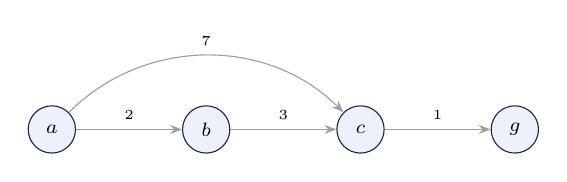
\begin{tikzpicture}[x=1.4cm,y=1cm]
			\node[st,minimum size=6mm,font=\scriptsize] (a) at (0,0) {$a$};
			\node[st,minimum size=6mm,font=\scriptsize] (b) at (1.4,0) {$b$};
			\node[st,minimum size=6mm,font=\scriptsize] (c) at (2.8,0) {$c$};
			\node[st,minimum size=6mm,font=\scriptsize] (g) at (4.2,0) {$g$};
			\draw[e] (a) -- node[above,font=\tiny]{2} (b);
			\draw[e] (b) -- node[above,font=\tiny]{3} (c);
			\draw[e] (c) -- node[above,font=\tiny]{1} (g);
			\draw[e] (a) to[bend left=45] node[above,font=\tiny]{7} (c);
		\end{tikzpicture}

		\small
		$V(g)=0$, all other $V=\infty$; update $V(s)\leftarrow\min_{s\to s'}\{w+V(s')\}$.

		\column{0.52\textwidth}
		\audience{Predict}{%
			\begin{enumerate}
				\item How many synchronous sweeps until $V(a)$ is final?
				\item Which update order finishes in one pass?
			\end{enumerate}
		}
	\end{columns}

	\uncover<2->{%
		\small
		(1) Three sweeps: information travels one edge per sweep. (2) $c,b,a$: a reverse topological order.
		The bottom-up evaluation of Part~1 is the \alert{best possible asynchronous schedule} when the graph is a DAG;
		for cyclic graphs, Dijkstra's priority queue computes such an order on the fly.%
	}
\end{frame}

\begin{frame}{Why asynchronous updates converge}
	\small
	\begin{theorem}[Bertsekas 1982; Bertsekas--Tsitsiklis 1989]
		Let $\Bell$ be a $\gamma$-contraction in $\supnorm\cdot$. If each coordinate is updated infinitely often, and
		stale information is eventually flushed, then $V_t\to v^\star$ for any initial $V_0$.
	\end{theorem}
	\begin{proof}[Box argument]
		Let $D=\supnorm{V_0-v^\star}$ and $B_k=\{V:\supnorm{V-v^\star}\le\gamma^kD\}$.
		Let $t_k$ be a time after which every coordinate has been updated at least once using only information from
		after $t_{k-1}$. Claim: $V_t\in B_k$ for $t\ge t_k$.
		Induction: an update of coordinate $s$ reads a vector in $B_{k-1}$, so
		$|V_{t+1}(s)-v^\star(s)|=|(\Bell V)(s)-(\Bell v^\star)(s)|\le\gamma\cdot\gamma^{k-1}D$, and further updates
		keep $s$ within the box.
	\end{proof}
	The per-coordinate contraction is all we need: no global clock, order, or synchronisation.
\end{frame}

\begin{frame}{From asynchronous DP to learning}
	\small
	Replace the expectation over $P$ by a \emph{sample} $(s,a,r,s')$ and take a step of size $\alpha_t$:
	\[
		Q(s,a)\leftarrow Q(s,a)+\alpha_t\Bigl[r+\gamma\max_{a'}Q(s',a')-Q(s,a)\Bigr].
	\]
	This is \alert{Q-learning}: asynchronous value iteration on $q^\star$ with stochastic approximation (Watkins--Dayan 1992; Tsitsiklis 1994).
	It converges when every pair $(s,a)$ is visited infinitely often and $\sum\alpha_t=\infty$, $\sum\alpha_t^2<\infty$.

	\seprule

	\begin{tabularx}{\textwidth}{@{}lX@{}}
		\toprule
		Carries over & Fixed point of the Bellman operator; contraction; state sufficiency; greedy extraction of the policy\\
		Changes & Model $P$ unknown (sampling replaces expectation); updates asynchronous by construction\\
		Breaks & With function approximation the composed operator need not be a contraction (Baird's counterexample)\\
		\bottomrule
	\end{tabularx}
\end{frame}

\begin{frame}{Discussion}
	\audience{Discuss}{%
		A state space with $10^{20}$ states (a board game, a robot with continuous sensors).
		\begin{enumerate}
			\item Which of the Part~1 requirements do you give up first?
			\item What replaces the table $V:\mathcal S\to\mathbb R$?
			\item Which guarantee from the contraction proof do you lose?
		\end{enumerate}
	}
\end{frame}

\section{Other Places, and What We Learned}

\begin{frame}{One DAG, many semirings}
	The recurrence $d(v)=\bigoplus_{u\to v}d(u)\otimes w(u,v)$ is a path problem over a semiring $(K,\oplus,\otimes)$.
	Changing the semiring changes the problem, not the algorithm.

	\small
	\begin{center}
		\renewcommand{\arraystretch}{1.15}
		\begin{tabularx}{\textwidth}{@{}llX@{}}
			\toprule
			$(\oplus,\otimes)$ & Computes & Examples\\
			\midrule
			$(\min,+)$ & shortest path & edit distance, Part~1\\
			$(\max,+)$ & longest path & Viterbi in log-space, critical path\\
			$(+,\times)$ & weighted path sum & domino tilings (Part~3), HMM forward algorithm\\
			$(\max,\times)$ & most probable path & Viterbi, probabilistic CYK\\
			$(\min,\max)$ & bottleneck path & Case~1 (split array), minimax routing\\
			$(\vee,\wedge)$ & reachability & parsing recognition, regular-expression matching\\
			\bottomrule
		\end{tabularx}
	\end{center}
\end{frame}

\begin{frame}{Name the semiring}
	\audience{Vote}{%
		Which semiring (if any) governs each recurrence?
		\begin{enumerate}
			\item[(a)] $N(i)=\sum_{j<i}N(j)\,[\,\text{edge }j\to i\,]$ (number of paths)
			\item[(b)] $f(i,j)=\min_p\max\{f(p,j-1),S_i-S_p\}$
			\item[(c)] $V_t(s)=\max_a\bigl[r+\sum_{s'}P(s'|s,a)V_{t+1}(s')\bigr]$
		\end{enumerate}
	}

	\uncover<2->{%
		\small
		(a) $(+,\times)$. (b) $(\min,\max)$. (c) \alert{None}: it alternates $\max$ over actions with an
		expectation over successors, so it is a path problem on an AND/OR graph (a hypergraph). For a \emph{fixed} policy
		it collapses to $(+,\times)$ and becomes linear: $v_\pi=r_\pi+\gamma P_\pi v_\pi$.
	}
\end{frame}

\begin{frame}{Linear optimisation: a staircase LP}
	\small
	\textbf{Production planning.} Periods $t=1,\dots,T$; demand $d_t$, unit production cost $c_t$, capacity $u$,
	unit holding cost $h$, inventory $s_t$ with $s_1$ given.
	\begin{align*}
		\min\quad & \sum_{t=1}^{T}\bigl(c_tx_t+h\,s_{t+1}\bigr)\\
		\text{s.t.}\quad & s_{t+1}=s_t+x_t-d_t, \qquad 0\le x_t\le u, \qquad s_{t+1}\ge0.
	\end{align*}
	This is an LP in $2T$ variables. Constraint $t$ involves only $(s_t,x_t,s_{t+1})$: a \alert{staircase} structure.
	Inventory $s_t$ is a sufficient state, and the LP is a path in a (continuous) state space:
	\[
		V_{T+1}\equiv0,\qquad
		V_t(s)=\min_{\substack{0\le x\le u\\ s+x-d_t\ge0}}\Bigl\{c_tx+h(s+x-d_t)+V_{t+1}(s+x-d_t)\Bigr\}.
	\]
	The state is real-valued: no table. What does $V_t$ look like?
\end{frame}

\begin{frame}{The value functions are piecewise linear and convex}
	\small
	\begin{columns}[T,onlytextwidth]
		\column{0.52\textwidth}
		\begin{tikzpicture}
			\begin{axis}[
				betterplot,
				width=\linewidth, height=5.2cm,
				xmin=0,xmax=7,ymin=0,ymax=13,
				xlabel={$s$},ylabel={$V_t(s)$},
				legend pos=north east, legend style={font=\scriptsize},
				]
				\addplot[plot0,thick,mark=*] coordinates {(0,12)(1,10)(2,8)(3,7)(4,6)(5,5)(6,6)(7,7)};
				\addplot[plot2,thick,mark=square*] coordinates {(0,11)(1,8)(2,5)(3,2)(4,2)(5,2)(6,4)(7,6)};
				\legend{$V_1$,$V_2$}
			\end{axis}
		\end{tikzpicture}

		\column{0.44\textwidth}
		\small
		$T=3$, $d=(2,3,2)$, $c=(1,3,1)$, $u=3$, $h=1$.

		\begin{theorem}
			Each $V_t$ is convex and piecewise linear on its domain.
		\end{theorem}
		\textit{Proof.} $V_t(s)$ is the optimal value of an LP whose right-hand side depends affinely on $s$;
		partial minimisation of a jointly convex polyhedral function over a polyhedron is convex and polyhedral.
		By induction, $V_{t+1}$ has the same form.
	\end{columns}

	\seprule

	\small DP is exact here without discretisation: represent $V_t$ by its breakpoints or its supporting lines (\emph{cuts}).
\end{frame}

\begin{frame}{Reading the slopes}
	\audience{Predict}{%
		$V_2$ has slope $-3$ on $[0,3]$, slope $0$ on $[3,5]$ and slope $+2$ on $[5,7]$.
		Explain each slope in terms of what one extra unit of inventory does.
	}

	\uncover<2->{%
		\small
		\begin{itemize}
			\item $[0,3]$: one extra unit avoids producing a unit at $c_2=3$ in period $2$: saving $3$.
			\item $[3,5]$: demand of period $2$ is covered; the extra unit then replaces production at $c_3=1$ in period $3$ but costs holding $h=1$: net $0$.
			\item $[5,7]$: all demand is covered; the extra unit is just held through periods $2$ and $3$: cost $2h=2$.
		\end{itemize}
		The slopes of $V_t$ are the LP \alert{dual variables} (shadow prices). Stochastic dual dynamic programming (SDDP)
		builds $V_t$ from exactly these supporting lines.
	}
\end{frame}

\begin{frame}{The other direction: MDPs as linear programs}
	\small
	For $\mu>0$ consider
	\[
		\min_v\;\sum_s\mu(s)v(s)\quad\text{s.t.}\quad v(s)\ge r(s,a)+\gamma\sum_{s'}P(s'|s,a)v(s')\quad\forall s,a.
	\]
	\textbf{Claim:} $v^\star$ is the unique optimum. Feasibility means $v\ge\Bell v$; by monotonicity of $\Bell$,
	$v\ge\Bell^kv\to v^\star$. So every feasible $v$ dominates $v^\star$, which is itself feasible.

	\seprule

	The dual variables $x(s,a)\ge0$ are \alert{discounted state-action occupancy measures}:
	\[
		\max_x\sum_{s,a}r(s,a)x(s,a)\quad\text{s.t.}\quad\sum_ax(s',a)-\gamma\sum_{s,a}P(s'|s,a)x(s,a)=\mu(s').
	\]
	Complementary slackness says $x(s,a)>0$ only if $a$ attains the maximum in the Bellman optimality equation.
	\textbf{Bellman optimality $=$ LP optimality conditions.}
\end{frame}

\begin{frame}{Dynamic programming elsewhere}
	\small
	\begin{center}
		\renewcommand{\arraystretch}{1.15}
		\begin{tabularx}{\textwidth}{@{}lX@{}}
			\toprule
			Area & Dynamic programming in disguise\\
			\midrule
			Computational biology & Needleman--Wunsch / Smith--Waterman alignment; RNA folding (Nussinov, Zuker)\\
			Language and speech & Viterbi decoding; CYK; inside--outside algorithm\\
			Probabilistic inference & Variable elimination / junction trees: DP over a tree decomposition of the model\\
			Optimal control & LQR: $V_t(x)=x^\top P_tx$ with the Riccati recursion for $P_t$\\
			Operations research & Multi-stage (stochastic) LPs and SDDP; DP-based algorithms for integer programs with small coefficients\\
			Economics & Recursive formulations of consumption and growth (Bellman equations over continuous states)\\
			\bottomrule
		\end{tabularx}
	\end{center}
\end{frame}

\begin{frame}{Your turn}
	\audience{Pair}{%
		Turn to your neighbour for three minutes. Pick a problem you work on.
		\begin{enumerate}
			\item What is a \textbf{sufficient state}? Is the state graph a DAG?
			\item Which \textbf{semiring} is it? What is the \textbf{edge count}?
			\item Which \textbf{lever} (recurrence, order, schedule) could reduce it?
		\end{enumerate}
		Then we collect two or three examples, including the ones that \emph{failed} the test.
	}
\end{frame}

\begin{frame}{What we learned}
	\begin{enumerate}
		\item \textbf{DP is path-finding in a state space.} A sufficient state and an acyclic order give a recurrence, and complexity is the number of edges.
		\item \textbf{Not every sequence of decisions is a DP.} Check for a compact sufficient state \emph{and} for cheaper structure (monotone decision problems, exchange arguments).
		\item \textbf{Speed comes from the shape of the DAG.} Rewrite the recurrence (convex hull trick) or refine the order (broken profile).
		\item \textbf{Beyond DAGs, DP is a fixed-point computation.} Bellman operators are contractions; value iteration, policy iteration and \emph{asynchronous} schedules are different ways of reaching the fixed point.
		\item \textbf{The reach is wide.} Semirings, linear programs, control and learning share the same recurrence.
	\end{enumerate}
\end{frame}

\begin{frame}[standout,plain]
	Questions and discussion
\end{frame}

\appendix

\begin{frame}{References (1/2)}
	\footnotesize
	\begin{itemize}
		\item R.~Bellman. \emph{Dynamic Programming}. Princeton University Press, 1957.
		\item D.~Bertsekas. Distributed dynamic programming. \emph{IEEE Trans.\ Automatic Control}, 1982.
		\item D.~Bertsekas, J.~Tsitsiklis. \emph{Parallel and Distributed Computation}. Prentice Hall, 1989.
		\item A.~Barto, S.~Bradtke, S.~Singh. Learning to act using real-time dynamic programming. \emph{Artificial Intelligence}, 1995.
		\item R.~Sutton, A.~Barto. \emph{Reinforcement Learning: An Introduction}, 2nd ed., MIT Press, 2018 (Ch.~3--4).
		\item M.~Puterman. \emph{Markov Decision Processes}. Wiley, 1994.
		\item Y.~Ye. The simplex and policy-iteration methods are strongly polynomial for the Markov decision problem with a fixed discount rate. \emph{Math.\ of Operations Research}, 2011.
		\item A.~Moore, C.~Atkeson. Prioritized sweeping. \emph{Machine Learning}, 1993.
	\end{itemize}
\end{frame}

\begin{frame}{References (2/2)}
	\footnotesize
	\begin{itemize}
		\item C.~Watkins, P.~Dayan. Q-learning. \emph{Machine Learning}, 1992; J.~Tsitsiklis. Asynchronous stochastic approximation and Q-learning. \emph{Machine Learning}, 1994.
		\item A.~Backurs, P.~Indyk. Edit distance cannot be computed in strongly subquadratic time (unless SETH is false). STOC 2015.
		\item E.~Myers. An $O(ND)$ difference algorithm and its variations. \emph{Algorithmica}, 1986.
		\item D.~Hirschberg. A linear space algorithm for computing maximal common subsequences. \emph{CACM}, 1975.
		\item M.~Pereira, L.~Pinto. Stochastic dual dynamic programming. \emph{Math.\ Programming}, 1991.
		\item R.~Larmore, B.~Schieber. On-line dynamic programming with applications to the prediction of RNA secondary structure. \emph{J.\ Algorithms}, 1991.
	\end{itemize}
\end{frame}

\begin{frame}{Backup: the Damerau--Levenshtein state}
	The unrestricted distance (Lowrance--Wagner) allows material to be edited between the two
	transposed symbols. For each $(i,j)$ let $i'<i$ be the last position with $x_{i'}=y_j$ and $j'<j$ the last
	position with $y_{j'}=x_i$ (when both exist). Add the edge
	\[
		(i'-1,j'-1)\to(i,j),\qquad \cost=(i-i'-1)+1+(j-j'-1),
	\]
	meaning: delete the gap in $x$, transpose, insert the gap in $y$.
	Time $O(mn)$ with $O(|\Sigma|)$ extra memory for the last-occurrence tables.
	The state is still $(i,j)$, but the \emph{edge set} reaches back arbitrarily far.
\end{frame}

\end{document}
